\documentclass[]{standalone}

\usepackage{pgfplots}
\usepackage{tikz}

\begin{document}

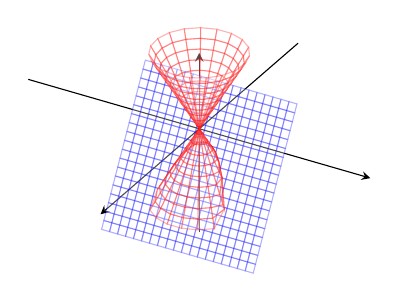
\begin{tikzpicture}
  \def\al{30}
  \def\phi{60}
  \def\tanal{tan(\al)}
  \def\h{-1.0}
    \begin{axis}[axis lines=center, ticks=none, view/h=120, view/v=30, xmin=-1, xmax=1, ymin=-1, ymax=1, axis equal,]
%   \addplot3+[domain=0:4*pi, samples=100, samples y=0, no marks, smooth, ultra thick,black](
%   {1+cos(deg(x))},
%   {sin(deg(x))},
%   {2*sin(deg(x)/2)}
%   );% node[blue,circle,fill,pos=0.3]{} node[red,draw,pos=0.65,thick]{};
%   \addplot3[%
%   opacity = 0.1,
%   mesh,
%   blue,
%   z buffer = sort,
%   samples = 10,
%   variable = \u,
%   variable y = \v,
%   domain = 0:180,
%   y domain = 0:360,
%   ]
%   ({2*cos(u)*sin(v)}, {2*sin(u)*sin(v)}, {2*cos(v)});
%   \addplot3[
%   opacity =0.3,
%   surf, % mesh,
%       faceted color=red,
%   white,
%   z buffer = sort,
%   samples = 16,
%   variable = \u,
%   variable y = \v,
%   domain = -135:135,
%   y domain = -2:2,
%   ]
%       ({\tanal*cos(u)*min(v,\h/(1+tan(\al)*tan(\phi)*cos(u))},{\tanal*sin(u)*min(v,\h/(1+tan(\al)*tan(\phi)*cos(u))},{min(v,\h/(1+tan(\al)*tan(\phi)*cos(u)))});
    \addplot3[%
    opacity =0.3,
    surf,  % mesh,
        faceted color=blue,
    white,
    z buffer = sort,
    samples = 20,
    variable = \u,
    variable y = \v,
    domain = -2:2,
    y domain = -2:2,
    ]
    ({v*cos(\phi)}, {u}, {\h-v*sin(\phi)});
    \addplot3[
    opacity =0.3,
    surf, % mesh,
        faceted color=red,
    white,
    z buffer = sort,
    samples = 20,
    variable = \u,
    variable y = \v,
    domain = 0:360,
    y domain = -2:2,
    ]
        ({\tanal*cos(u)*max(v,\h/(1+tan(\al)*tan(\phi)*cos(u))},{\tanal*sin(u)*max(v,\h/(1+tan(\al)*tan(\phi)*cos(u))},{max(v,\h/(1+tan(\al)*tan(\phi)*cos(u)))});
  \end{axis}
\end{tikzpicture}

\end{document}
